%%%%%%%%%%%%%%%%%%%%%%%%%%%%%%%%%
%%  Descrizione dell'architettura
%%%%%%%%%%%%%%%%%%%%%%%%%%%%%%%%%



\subsection{Metodo e formalismo di specifica}
Suddividiamo la descrizione dell'architettura di \proj{} in quattro sezioni:
\begin{itemize}
	\item §\ref{sec:arch_gen}, che illustra gli aspetti generali dell'architettura del software;
	\item §\ref{sec:arch_client}, che descrive l'architettura del \emph{front end} dell'applicazione;
	\item §\ref{sec:arch_server}, che descrive l'architettura del \emph{back end} dell'applicazione;
	\item §\ref{sec:arch_proto}, che descrive il protocollo che lega le due interfacce precedenti.
\end{itemize}
Per ognuna di queste sezioni, descriviamo l'architettura con metodo \emph{top-down} --- dal generale al particolare --- utilizzando i formalismi di UML 2.0.



\subsection{Architettura generale} \label{sec:arch_gen}
L'architettura dell'applicazione è suddivisa in due moduli:
\begin{enumerate}
	\item il client, che vive nel browser dell'utente;
	\item il server, che fornisce la pagina dell'applicazione al client e riceve da esso delle richieste di generazione di codice.
\end{enumerate}

Tra le varie qualità desiderabili per la nostra architettura, la progettazione ha cercato di perseguire principalmente l'\textbf{estensibilità}. Tale obiettivo è stato perseguito in due modi:
\begin{itemize}
	\item in generale, promuovendo le seguenti qualità:
	\begin{itemize}
		\item manutenibilità;
		\item modularità;
		\item semplicità;
		\item basso accoppiamento.
	\end{itemize}
	\item nello specifico, prevedendo le seguenti possibili aggiunte nel futuro:
	\begin{itemize}
		\item Generazione di codice in altri linguaggi target: se i manutentori vorranno generare del \gloss{JavaScript} o del Python, sarà sufficiente aggiungere dei template per il linguaggio scelto (grazie alla libreria StringTemplate).
		\item Diverso formato per i diagrammi in input: si potrebbe voler ricevere dei dati in XML, anziché in JSON; sarà sufficiente implementare l'interfaccia \texttt{Generator} con una nuova classe concreta, da fornire al controller.
		\item Diversa compressione del codice generato: attualmente l'applicazione genera codice Java e lo fornisce in formato ZIP, ma si potrebbe facilmente cambiare il formato di compressione in TAR o JAR.
		\item Persistenza dei dati del diagramma che arrivano in input al \emph{back end}: si potrebbe voler mantenere un database di utenti dell'applicazione, ognuno con i propri diagrammi mantenuti nel server a tempo indefinito; oppure; per questo, basta fornire l'indirizzo della risorsa JSON, che attualmente non viene eliminata dal server. % (oppure per ora potremmo eliminarla...)
		\item Persistenza del programma generato: si potrebbe voler mantenere anche il codice generato, come il diagramma di input; per fare ciò, basta garantire al client il carattere persistente della risorsa fornita (badando però a non eliminarla dal server). % (per ora la eliminiamo?)
	\end{itemize}
\end{itemize}



\subsection{Architettura del client} \label{sec:arch_client}
Il \emph{front end} di \proj{} è una singola pagina web scritta in HTML5, CSS3 e JavaScript.

L'\texttt{head} (intestazione, invisibile) della pagina HTML contiene dei puntatori a:
\begin{itemize}
	\item le librerie JavaScript elencate nella sezione \ref{sec:tech_client} (con eventuali relativi fogli CSS);
	\item il foglio di stile CSS della pagina;
	\item lo script JavaScript che utilizza le librerie di cui sopra.
\end{itemize}

Il \texttt{body} (corpo, visibile) della pagina HTML si compone di pochi blocchi:
\begin{itemize}
	\item dei tag \texttt{div} contenenti i menù laterali da cui selezionare gli strumenti e gli elementi per interagire con i diagrammi;
	\item un tag \texttt{canvas} (identificato dall'\texttt{id} \emph{paper}) che contiene, di volta in volta, il diagramma delle classi o il diagramma di un metodo particolare.
\end{itemize}

Alla ricezione della pagina da parte del client, il nostro script JavaScript popola il tag \texttt{canvas} (inizialmente vuoto) con un diagramma delle classi vuoto.

%%% [...]



\subsection{Architettura del server} \label{sec:arch_server}
Il server offre due servizi:
\begin{enumerate}
	\item fornisce al client la pagina HTML dove disegnare i diagrammi;
	\item elabora un file JSON in arrivo dal client e gli fornisce l'applicazione generata a partire da tale file.
\end{enumerate}
Questi due servizi rispettano lo stile architetturale REST, come spiegato nella sezione \ref{sec:arch_proto}.

Il \emph{back end} del server è suddiviso nei seguenti due moduli (penso):
\begin{itemize}
	\item controller: rappresenta il core del \emph{back end}; si occupa di ricevere ed elaborare le richieste provenienti dal client.
	\item endpoints: per la REST (ce l'abbiamo???)
\end{itemize}



\subsection{Protocollo di comunicazione client-server} \label{sec:arch_proto}
I due servizi offerti dal server (ottenere la pagina HTML e ottenere l'applicazione generata) seguono lo stile architetturale REST:
\begin{itemize}
	\item La richiesta per ottenere la pagina HTML usa il metodo HTTP GET; la pagina è quindi \emph{cachable} (i router tra client e server possono decidere di ottimizzarne la fornitura).
	\item Il file JSON viene spedito con il metodo HTTP POST, che permette la persistenza di tale file nel server; la persistenza del file JSONè indifferente alla nostra applicazione ma ne aumenta l'estensibilità, in quanto un giorno i manutentori potrebbe voler offrire un servizio di condivisione dei diagrammi disegnati oppure un database di utenti che abbiano i propri diagrammi sul server.
	\item Ognuno dei due servizi (la pagina HTML e la generazione di codice) è una risorsa distinta: questo disaccoppia i due servizi, aumentando ancora la manutenibilità del sistema.
	\item La richiesta per ottenere la pagina HTML è per forza idempotente: lo stato del server non può influire su una pagina statica.
	\item La richiesta di generazione di codice è idempotente: l'unica dipendenza esterna al programma è il file JSON, che viene passato dal client.
\end{itemize}

\begin{center}
	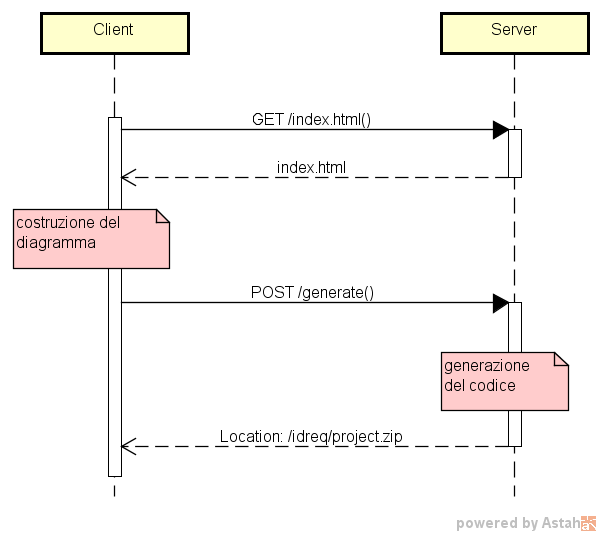
\includegraphics[scale=0.5]{img/http}
\end{center}
